\documentclass[journal,a4paper]{IEEEtran}
\usepackage{kotex}
\XeTeXlinebreaklocale ""
\setmainhangulfont{NanumMyeongjo}
\setsanshangulfont{NanumGothic}
\usepackage{amsmath,amssymb,bm}
\usepackage{booktabs,array}
\newcolumntype{L}[1]{>{\raggedright\arraybackslash}p{#1}}
\usepackage{graphicx}
\usepackage{url}
\usepackage{multirow}
\usepackage[hidelinks]{hyperref}
\newcommand{\Normal}{\mathcal{N}}
\renewcommand{\abstractname}{초록}
\renewcommand{\IEEEkeywordsname}{주제어}
\renewcommand{\tablename}{표}
\renewcommand{\figurename}{그림}
\renewcommand{\refname}{참고문헌}
\linespread{1.04}
\raggedbottom

\title{CREDO: BC카드 소비 데이터 기반\\불확실성 인지형 창업 최적입지 판단 모델}
\author{CREDO 팀}

\begin{document}
\maketitle

\begin{abstract}
BC카드 결제 데이터로 창업 입지를 고르면 세 가지 착시가 생긴다. 비식별 억제로 작은 시장이 사라지고 균형 결과인 점포당 매출이 미충족 수요로 오인되며 순위표는 틀릴 확률을 알려주지 않는다. 본 연구는 전국 255개 시군구와 8개 업종에서 이 세 가지를 차례로 바로잡는 CREDO(Confidence-Robust Demand Opportunity)를 제안한다. 층 1은 억제 셀을 검열 우도로 복원하는 계층 베이지안 음이항 수요모형이다. 층 2는 비슷한 수요·비용·유입 조건의 지역보다 점포가 얼마나 적은지를 자유진입 회귀로 추정하고 지역 안 업종 간 상대값 $\tilde R$로 BC카드 점유율 차이를 상쇄한다. 층 3은 사후기대 오탐률(FDR), 지식 기울기, 부분모듈 공간 커버리지를 써서 개설 후보·4주 검증·보류를 정한다. 억제 셀 5,041개를 포함한 161,136셀을 적합한 결과, 명목 90\% 예측구간의 실제 포함률은 90\%--91\%였다. 업종마다 오탐률 10\% 이하인 개설 후보가 58--67곳 선정되었고 전국 17개 시도 모두에 후보가 있다. 과거 자료를 쓴 사후 점검에서 $\tilde R$은 신규 점포 1년 생존과 양의 순위상관(+0.075)을 보였고 그 값은 점포 수만 보는 기준보다 +0.043--+0.118 높았다.
\end{abstract}

\begin{IEEEkeywords}
계층 베이지안 모형, 검열 음이항 우도, 자유진입 모형, 사후기대 FDR, 지식 기울기, 최적입지 선정
\end{IEEEkeywords}

\section{서론}
예비창업자와 소상공인 지원기관은 가장 먼저 ``이 지역에서 이 업종을 열면 살아남을까''를 묻는다. 카드 결제 데이터는 이 질문에 답할 수 있는 드문 전국 단위 자료지만 그대로 순위를 매기면 세 가지 착시에 빠진다.

첫째, \textbf{사라진 작은 시장}이다. 제공 데이터 242,574행에서 거래건수 최솟값은 모든 업종·성별·월에서 정확히 11이다. 10건 이하 셀은 비식별 처리로 삭제되어 격자의 약 24\%가 비어 있다. 이 빈 셀을 0으로 보거나 버리면 작은 시장의 수요가 체계적으로 과소평가된다.

둘째, \textbf{점포당 매출은 부족의 증거가 아니다}. 자유진입 균형에서 점포당 매출은 손익분기 수준에 가깝다\cite{BerryWaldfogel1999}. 흔히 쓰는 ``점포당 수요 $G=\log D-\log(S+1)$''는 임대료가 비싸 점포가 적은 곳, 유입 인구가 많은 곳, BC카드 점유율이 높은 곳에서 모두 커진다.

셋째, \textbf{순위표는 틀릴 확률을 알려주지 않는다}. 상위 $N$곳 목록만으로는 그중 몇 곳이 우연히 올라왔는지 알 수 없고 임의로 정한 임계값도 방어하기 어렵다.

입지 선택과 점포 수의 관계는 산업조직론의 진입 문턱 모형에서 오래 다뤄졌다. 이 모형에서는 시장 규모가 커질 때 점포 수가 얼마나 늘어나는지로 경쟁 강도와 진입 조건을 추정하며\cite{Bresnahan1991,Schaumans2015}, 실제 진입·퇴출과의 연관도 검증되었다\cite{Carree2007}. 계층 모형의 순위 추정에서는 사후평균으로 순위를 매기면 수축 때문에 극단 순위가 왜곡되므로 앙상블 분포와 순위 손실함수를 쓰는 방법이 제안되었다\cite{ShenLouis1998,Lin2006}. 다중 판단에서는 사후기대 오탐률로 목록 크기를 정하는 결정이론적 규칙이\cite{Muller2004}, 추가 관측의 가치를 따질 때는 지식 기울기가\cite{Frazier2008}, 예산 제약 선택에서는 부분모듈 함수의 탐욕 근사가\cite{Nemhauser1978} 표준이다. 통계데이터 활용대회에서도 카드 데이터로 수요와 공급을 맞춰 입지를 추천해 수상한 사례가 있다. 기존 연구와 달리 본 연구는 이 도구들을 억제된 카드 집계 데이터를 다루는 하나의 흐름으로 묶어 순위가 아닌 판단과 그 오류율을 내놓는다.

본 연구의 기여는 네 가지다. (i) 억제 셀을 ``10건 이하''라는 구간 정보로 우도에 넣어 복원한다. (ii) 수요·비용·유입을 통제한 뒤 남는 점포 부족을 \emph{시장 여유}로 정의하고 기존 지표 $G$가 그 특수해임을 보인다. (iii) 개설·검증·보류를 사후기대 FDR\cite{Muller2004}, 지식 기울기\cite{Frazier2008}, 공간 커버리지로 유도한다. (iv) 결과를 전국 최적입지 선정표와 서비스 화면으로 구체화하고 판단표를 사전 등록해 향후 자료로 검증한다.

\section{데이터}
\subsection{BC카드 제공 데이터에서 확인한 사실}
표~\ref{tab:facts}에 원자료를 직접 분석해 확인한 사실과 이를 모형에 반영한 방식을 정리했다. 지역 구분은 거주지가 아니라 가맹점 소재지 기준으로 판단된다. 주민 1인당 한식 결제 건수가 부산 중구 19.7건, 화성 동탄구 1.3건으로 도심에서 크게 튀기 때문이다.

\begin{table}[t]
\centering
\caption{BC카드 제공 데이터에서 확인한 사실}
\label{tab:facts}
{\footnotesize\setlength{\tabcolsep}{3pt}
\begin{tabular}{L{0.16\linewidth}L{0.36\linewidth}L{0.38\linewidth}}
\toprule
항목 & 확인 내용 & 모형 반영 \\\midrule
억제 기준 & cnt 최솟값 11 (업종·성별·월 전부) & $C=\min(\mathrm{cnt})-1=10$, 검열 우도 \\
지역 기준 & 가맹점 소재지 & 인구는 노출량, 유입은 공변량 \\
업종 & 한정식 관측률 2.8\%, 갈비 14.3\% & 일반한식과 합산해 한식 \\
대형할인점 & 57개 군은 전 기간 거래 없음 & 존재 조건부 수요, 지원금 대조군 \\
코드 & 성별·연령 x는 누락(법인 아님) & 국내 개인만 사용 \\
\bottomrule
\end{tabular}}
\end{table}

\subsection{결합한 외부 데이터}
표~\ref{tab:ext}의 공공 데이터 7종을 255개 시군구 단위로 결합했다. 모든 결합에는 시도명과 시군구명을 묶은 복합키를 썼다. 시군구명만 쓰면 서로 다른 이름이 233개뿐이라 255개 시군구를 구분하지 못한다.

\begin{table}[t]
\centering
\caption{결합한 외부 데이터}
\label{tab:ext}
{\footnotesize\setlength{\tabcolsep}{3pt}
\begin{tabular}{L{0.44\linewidth}L{0.2\linewidth}L{0.28\linewidth}}
\toprule
데이터 & 기준 & 모형 역할 \\\midrule
행정안전부 주민등록 인구(성·연령) & 2026-06 & 수요 노출량 $P$ \\
국세청 100대 생활업종 사업자 수 & 2026-06 & 공급 $S$ \\
한국관광공사 기초지자체 방문자수 & 2026-01--06 & 유입 수요 $x$, $w$ \\
국민연금 가입 사업장 가입자수 & 2026-07 & 주간 근로인구 $w$ \\
국토교통부 아파트 매매 실거래가 & 2026-01--06 & 임대료 대리 $w$ \\
소상공인 상가(상권)정보 4개 시점 & 2023--2026 & 상권 중심점, 사후 점검 \\
고유가 피해지원금 지역 등급 & 2026-04--08 & 5--6월 교란 통제 \\
\bottomrule
\end{tabular}}
\end{table}

\subsection{결합 과정에서 바로잡은 오류}
2026년 7월 행정구역 개편으로 외부 자료의 명칭이 공모전 데이터와 달랐다. 그대로 결합하면 30개 시군구가 빠지고 인천 서구는 잔여 행(사업자 20곳)에 붙어 실제 38,693곳이 20곳으로 잡힌다. 이 경우 점포당 수요 지표가 최상위로 튀는 전형적인 실패가 생긴다. 법정동 코드로 개편을 되돌리고 제물포구는 옛 동구 법정동 비율(0.406)로 나눈 뒤, 사업자 수 합계가 보존되는지를 검사 항목으로 고정했다.

\section{방법}
시군구 $i$, 성·연령 $g$, 업종 $b$, 월 $t$에 대해 세 층을 차례로 추정한다. 층 2는 층 1 사후표본을 조건으로 받는 단방향(cut) 구조이며 불확실성은 사후 draw 단위로 전파된다.

\subsection{층 1: 억제를 복원하는 수요모형}
\begin{figure}[t]
\centering
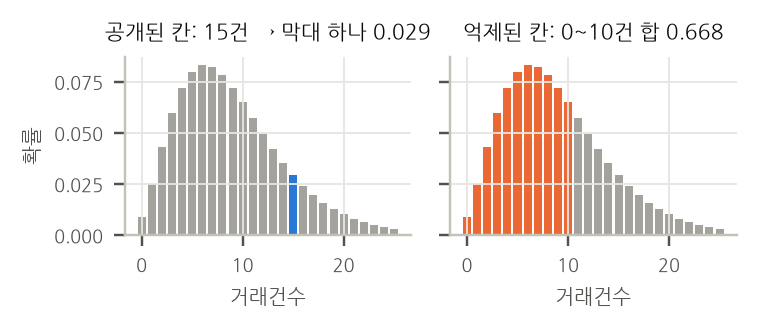
\includegraphics[width=\linewidth]{figures/concept_censor.png}
\caption{검열 우도의 개념 예시(음이항 $\mu=9$, $\phi=4$). 공개된 칸은 관측값의 확률 하나를, 억제된 칸은 0--10건 확률의 합을 쓴다.}
\label{fig:censor}
\end{figure}
관측 셀과 억제 셀의 우도는
\begin{align}
\Pr(Y_{igbt}=y)&=\mathrm{NB}(y\mid\mu_{igbt},\phi_b),\quad y\ge C+1 \label{eq:lik}\\
\Pr(Y_{igbt}\le C)&=\textstyle\sum_{k=0}^{C}\mathrm{NB}(k\mid\mu_{igbt},\phi_b)\nonumber
\end{align}
이다. 억제 셀은 ``0부터 $C$ 사이 어딘가''라는 정보만 주므로 우도에서는 해당 막대의 확률을 모두 더한다(그림~\ref{fig:censor}). 억제 셀을 버리면 작은 시장이 통째로 빠져 수요가 부풀려지지만 이처럼 우도에 넣으면 ``작다''는 정보가 남는다. 기대 거래건수는
\begin{multline}
\log\mu_{igbt}=\log P_{ig}+\log n_t+\alpha_b+\gamma_{bg}+\tau_{bt}\\
+e_b\,\delta_{tk(i)}+x_{it}^{\top}\beta_b+u_i+v_{ib}
\label{eq:eta}
\end{multline}
로 둔다. $P$는 인구, $n_t$는 월 일수, $\tau_{bt}$는 업종별 계절성, $\delta_{tk}$는 월$\times$지원금 등급 효과다. $e_b$는 지원금 적격 업종이면 1, 대형할인점이면 0이어서 대형할인점이 지원금 효과의 대조군 역할을 한다. $x_{it}$는 월별 방문자 변동, $u_i$와 $v_{ib}$는 지역과 지역$\times$업종 효과(합-0 제약)다. 16만 셀을 GPU NUTS\cite{Hoffman2014}로 적합하고 6개월 수요 $D_{ib}$의 사후 draw 1,000개를 다음 층으로 넘긴다.

\subsection{층 2: 자유진입 조건의 시장 여유}
점포 수는 계수 자료이므로 과산포를 보정한 포아송 회귀를 쓴다.
\begin{align}
\log E[S_{ib}]&=a_b+\psi_b\log D^{c}_{ib}+w_i^{\top}\rho_b, \label{eq:supply}\\
D^{c}_{ib}&=\textstyle\sum_j e^{-d_{ij}/\lambda}D_{jb}\nonumber
\end{align}
$w_i$는 아파트 ㎡가, 국민연금 가입자, 평균 방문자다. 한식·중식·일식·서양처럼 멀리서도 찾아가는 목적형 업종에는 $\lambda=10$km 거리 감쇠로 주변 수요를 합치고 편의점·슈퍼·제과·스넥 같은 근린형에는 자기 지역 수요만 쓴다. 시장 여유와 상대 시장 여유는
\begin{equation}
R_{ib}=\log\hat S_{ib}-\log(S_{ib}+0.5),\qquad
\tilde R_{ib}=R_{ib}-\frac{1}{8}\sum_{b'}R_{ib'}
\label{eq:slack}
\end{equation}
이다. $R>0$이면 비슷한 조건의 지역보다 점포가 적다. 기존 지표 $G$는 $\psi_b=1$, $\rho_b=0$인 특수해다. BC카드 점유율 $s_i$가 지역마다 다르면 $\log D_{ib}$에 $\log s_i$가 업종 공통으로 더해져 $R_{ib}$에 $\psi_b\log s_i$가 섞인다. 지역 안 업종 평균을 빼면 이 성분이 상쇄되고 $(\psi_b-\bar\psi)\log s_i$만 남는다. 실제로 $R$ 분산의 45.5\%가 시군구 공통 성분이었다. 이 성분에서는 점유율 편향과 지역 전체 과소공급을 데이터로 구분할 수 없으므로 판단에 쓰지 않는다. 그림~\ref{fig:rel}에서 절대 $R$의 지역 평균이 가장 높은 곳과 낮은 곳의 실제 결과를 비교했다. 절대 $R$로는 한 지역의 모든 업종이 한꺼번에 높거나 낮게 나오지만 $\tilde R$로 바꾸면 그 지역 안에서 상대적으로 모자란 업종만 위로 남는다.

\begin{figure}[t]
\centering
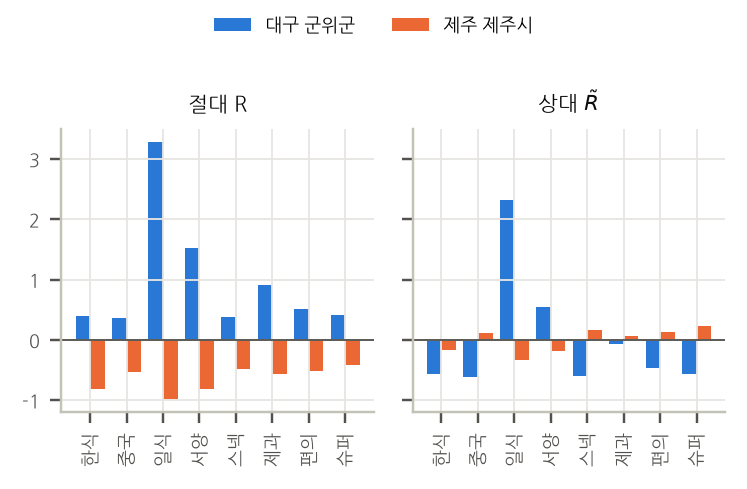
\includegraphics[width=\linewidth]{figures/concept_relative.png}
\caption{절대 시장 여유 $R$과 상대 시장 여유 $\tilde R$(사후평균). 절대 $R$의 지역 평균이 가장 높은 곳과 낮은 곳의 실제 값이다.}
\label{fig:rel}
\end{figure}

\subsection{층 3: 판단 규칙}
\subsubsection{기준선과 확률}
업종별로 모든 지역의 사후분포를 합친 앙상블 분포에서 75\% 분위를 기준선으로 둔다\cite{ShenLouis1998}.
\begin{equation}
\bar G_b(r)=\frac{1}{255}\sum_j\Pr(\tilde R_{jb}\le r\mid y),\quad r_\gamma=\bar G_b^{-1}(0.75)
\end{equation}
지역별 사후평균으로 분위수를 구하면 수축 때문에 분포가 좁아져 기준선이 낮게 잡히므로 앙상블 분위수를 쓴다. 판단의 근거가 되는 확률은 $v_{ib}=\Pr(\tilde R_{ib}>r_\gamma\mid y)$, 즉 상위 25\%에 들 확률이다.

\subsubsection{개설 후보: 사후기대 FDR}
$v$가 높은 순으로 목록을 늘리면서 평균 오탐 확률이 10\%를 넘기 직전에 멈춘다\cite{Muller2004}.
\begin{equation}
D^{*}=\max\Bigl\{D:\tfrac{1}{D}\textstyle\sum_{k\le D}\bigl(1-v_{(k)}\bigr)\le 0.10\Bigr\}
\label{eq:fdr}
\end{equation}
이 규칙은 목록 길이를 데이터로 정하고 ``추천 목록의 기대 오탐률 10\% 이하''라는 약속을 붙인다. 기존의 고정 임계값 0.8은 오탐 비용이 미탐의 4배라는 가정과 같다. 한식에서 이 규칙이 목록 길이를 정하는 과정을 그림~\ref{fig:fdr}에 나타냈다.

\begin{figure}[t]
\centering
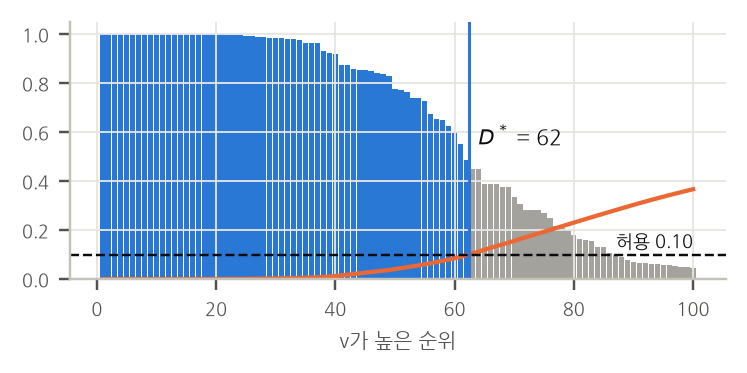
\includegraphics[width=\linewidth]{figures/concept_fdr.png}
\caption{한식의 FDR 목록 길이 결정(실제 결과). 막대는 $v$가 높은 순의 지역, 선은 1위부터 $D$위까지의 평균 오탐 확률 $\frac{1}{D}\sum(1-v)$.}
\label{fig:fdr}
\end{figure}

\subsubsection{4주 검증: 지식 기울기}
개설 후보 밖에서 팝업 한 번으로 판단이 뒤집힐 가능성이 큰 곳을 고른다\cite{Frazier2008}.
\begin{align}
\nu_{ib}&=\tilde\sigma f\Bigl(-\frac{|\mu_{ib}-r_\gamma|}{\tilde\sigma}\Bigr),\quad f(z)=z\Phi(z)+\varphi(z),\\
\tilde\sigma&=\sigma_{ib}^2\big/\sqrt{\sigma_{ib}^2+\lambda_p}\nonumber
\end{align}
기준선에 가깝고 불확실성이 큰 곳일수록 $\nu$가 크다. $\lambda_p$는 팝업 관측오차다. 업종마다 $\nu$ 상위 10곳을 검증 후보로 둔다. 그림~\ref{fig:kg}처럼 실제로 검증 후보는 기준선에 가깝고 사후 표준편차가 큰 영역에 모인다.

\begin{figure}[t]
\centering
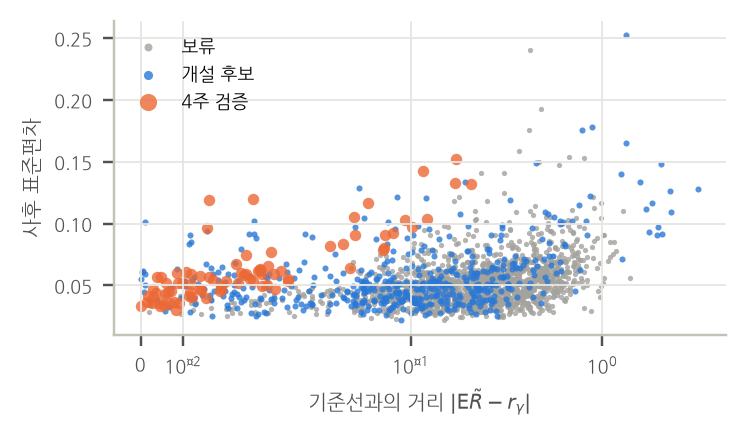
\includegraphics[width=\linewidth]{figures/concept_kg.png}
\caption{8개 업종 2,040개 판단의 기준선 거리 $|\mathrm{E}\tilde R-r_\gamma|$와 사후 표준편차. 4주 검증 후보는 가깝고 불확실한 곳에 모인다.}
\label{fig:kg}
\end{figure}

\subsubsection{최적입지 선정: 공간 커버리지}
지원기관이 $K$곳을 고를 때 인접 지역이 중복되지 않도록
\begin{equation}
\max_{|X|=K}E\Bigl[\sum_j\tilde R^{+}_{jb}\max_{i\in X}c_{ij}\Bigr],\quad
c_{ij}=\begin{cases}\mathbf 1[i=j] & \text{근린형}\\ e^{-d_{ij}/10\mathrm{km}} & \text{목적형}\end{cases}
\label{eq:cover}
\end{equation}
를 개설 후보 안에서 푼다. 목적함수가 단조 부분모듈이므로 탐욕법이 $(1-1/e)$ 근사를 보장한다\cite{Nemhauser1978}. 커버 비율은 사후 draw마다 계산해 구간으로 보고한다.

\section{결과: 전국 최적입지}
\subsection{업종별 판단과 전국 분포}
업종별 판단 수와 공간 커버 비율을 표~\ref{tab:counts}에 제시했다. 업종마다 개설 후보 58--67곳(합계 500건), 4주 검증 10곳이 선정되었다. 그림~\ref{fig:heat}처럼 후보는 수도권에만 몰리지 않고 17개 시도 전부에 분포한다. 시도마다 시군구 수가 달라 색으로는 개설 후보 비율을, 숫자로는 개수를 표시했다.


\begin{table}[t]
\centering
\caption{업종별 판단 수와 공간 커버 비율}
\label{tab:counts}
{\footnotesize\begin{tabular}{lrrrrr}\toprule
업종 & 개설 & 검증 & 보류 & 커버 K=10 & 커버 K=20 \\\midrule
한식 & 62 & 10 & 183 & 39\% & 56\% \\
중국음식 & 63 & 10 & 182 & 38\% & 55\% \\
일식회집 & 67 & 10 & 178 & 32\% & 48\% \\
서양음식 & 65 & 10 & 180 & 36\% & 52\% \\
스넥 & 60 & 10 & 185 & 30\% & 46\% \\
제과점 & 58 & 10 & 187 & 27\% & 44\% \\
편의점 & 62 & 10 & 183 & 24\% & 42\% \\
슈퍼마켓 & 63 & 10 & 182 & 22\% & 38\% \\\bottomrule\end{tabular}}
\vspace{2pt}

{\scriptsize 커버 = 개설 후보 중 $K$곳을 골랐을 때 전국 양(+)의 시장 여유를 덮는 사후평균 비율.}
\end{table}

\begin{figure}[t]
\centering
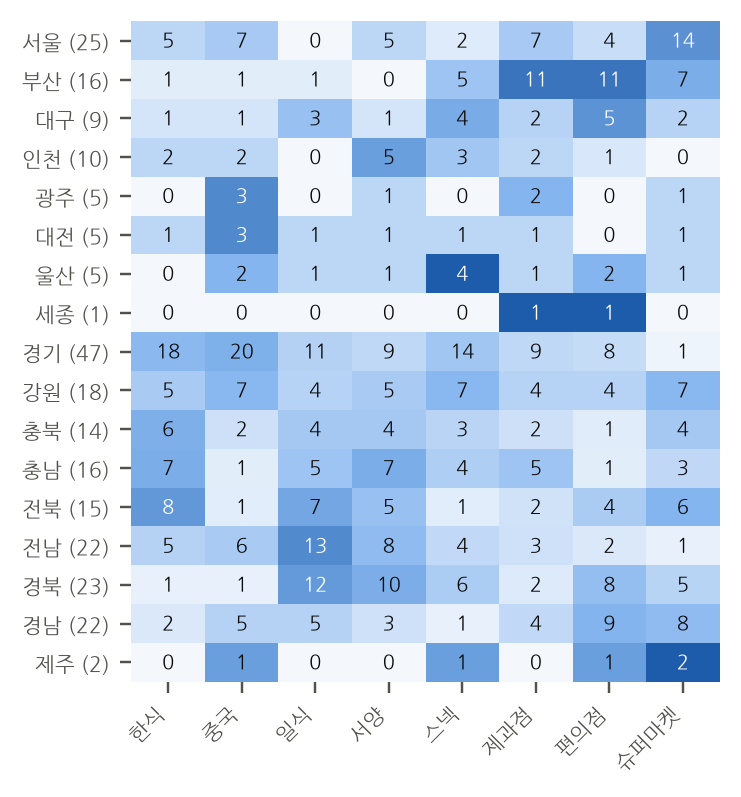
\includegraphics[width=\linewidth]{figures/sido_heatmap.png}
\caption{시도별 개설 후보. 색은 시도 내 시군구 대비 후보 비율, 숫자는 후보 수, 괄호는 시군구 수.}
\label{fig:heat}
\end{figure}

\subsection{업종별 최적입지 선정 순서}
식~\eqref{eq:cover}의 탐욕 선정으로 얻은 업종별 최적입지 1--5순위를 표~\ref{tab:picks}에 정리했다. 목적형 업종에서는 10km 안에서 서로 겹치지 않는 지역을, 근린형 업종에서는 시장 여유가 큰 지역부터 차례로 고른다. 한식에서 10곳을 고르면 전국 한식 시장 여유의 38.5\%(90\% 구간 32.7\%--43.8\%)를 덮는다.

목적형인 한식과 근린형인 편의점은 1--10순위를 시군구 경계 지도에 직접 표시했다(그림~\ref{fig:optH}, \ref{fig:optC}). 최적입지가 몰린 두 권역은 확대 창으로 따로 보였다. 한식은 수도권·충청·전북·전남·강원에 흩어져 선택되지만 편의점은 10곳 중 8곳이 부산과 대구 도심에 몰린다. 목적형은 10km 상권이 겹치지 않도록 떨어진 곳을 고르고, 근린형은 자기 지역만 커버하므로 인접 자치구가 함께 선택될 수 있어서다.

\begin{figure*}[t]
\centering
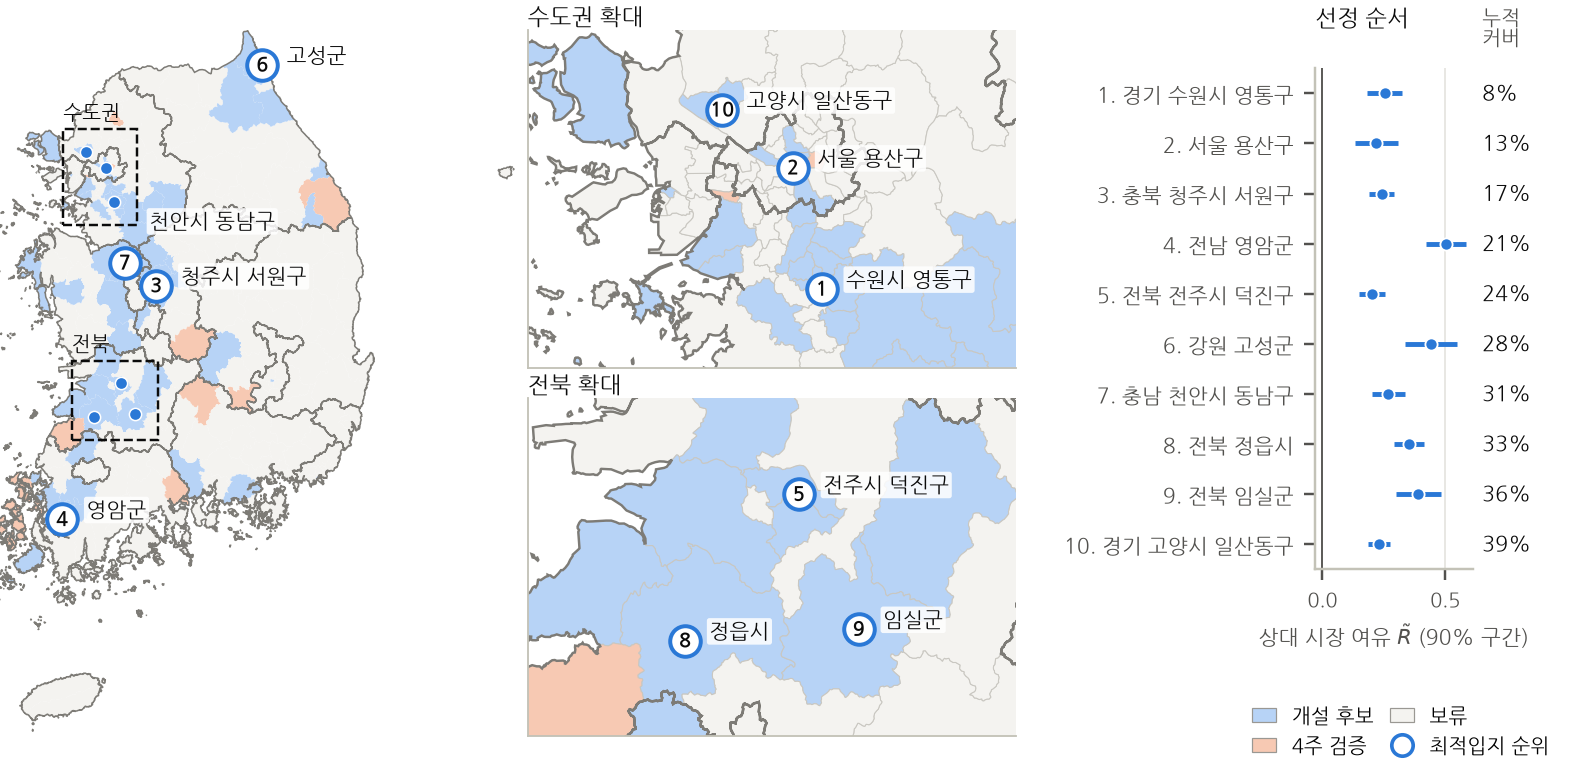
\includegraphics[width=\textwidth]{figures/optimal_H.png}
\caption{한식 최적입지 1--10순위. 왼쪽은 전국 판단 지도, 가운데는 최적입지가 몰린 두 권역의 확대 창, 오른쪽은 선정 순서별 상대 시장 여유 $\tilde R$(90\% 구간)과 누적 커버 비율이다. 경계: 통계청 SGIS(가공 vuski/admdongkor, CC BY 4.0).}
\label{fig:optH}
\end{figure*}

\begin{figure*}[t]
\centering
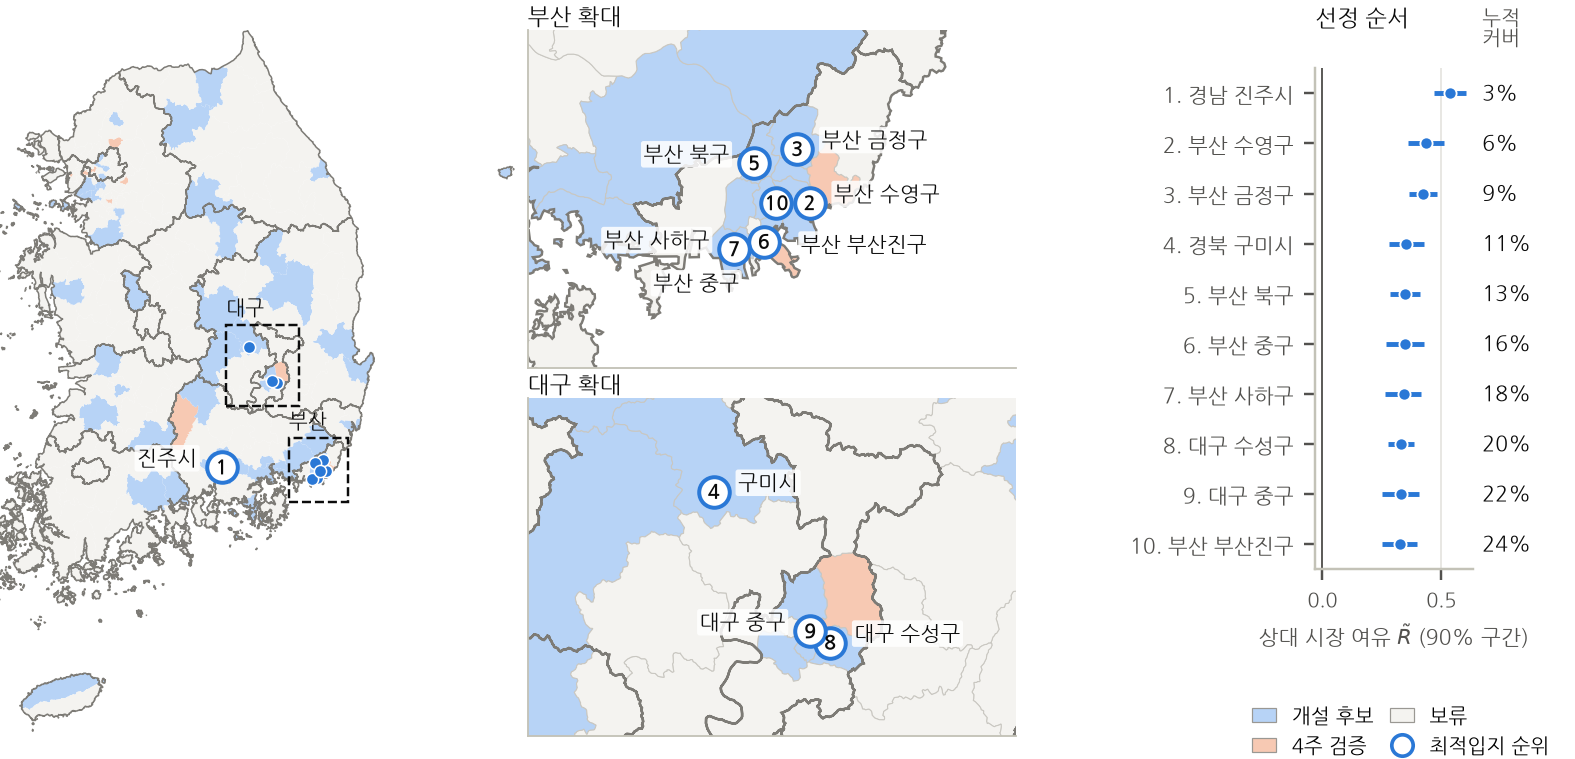
\includegraphics[width=\textwidth]{figures/optimal_4010.png}
\caption{편의점 최적입지 1--10순위. 구성은 그림~\ref{fig:optH}와 같다.}
\label{fig:optC}
\end{figure*}

\begin{table*}[t]
\centering
\caption{업종별 최적입지 선정 순서 (공간 커버리지 탐욕 선정, 커버는 5곳 기준)}
\label{tab:picks}
{\scriptsize\begin{tabular}{llllllr}\toprule
업종 & 1순위 & 2순위 & 3순위 & 4순위 & 5순위 & 커버 \\\midrule
한식 & 경기 수원시 영통구 & 서울 용산구 & 충북 청주시 서원구 & 전남 영암군 & 전북 전주시 덕진구 & 24\% \\
중국음식 & 경기 과천시 & 서울 중구 & 충남 계룡시 & 경기 용인시 기흥구 & 광주 남구 & 26\% \\
일식회집 & 전남 곡성군 & 전북 무주군 & 전남 함평군 & 대구 군위군 & 경남 의령군 & 18\% \\
서양음식 & 전남 완도군 & 경기 부천시 소사구 & 전북 장수군 & 경북 영양군 & 전남 신안군 & 25\% \\
스넥 & 충북 괴산군 & 충북 음성군 & 강원 강릉시 & 강원 속초시 & 경북 성주군 & 19\% \\
제과점 & 대전 중구 & 전남 보성군 & 강원 양양군 & 울산 동구 & 부산 영도구 & 16\% \\
편의점 & 경남 진주시 & 부산 수영구 & 부산 금정구 & 경북 구미시 & 부산 북구 & 13\% \\
슈퍼마켓 & 강원 횡성군 & 제주 서귀포시 & 전북 정읍시 & 부산 수영구 & 서울 금천구 & 12\% \\\bottomrule\end{tabular}}
\end{table*}

\subsection{전국 상위 입지}
업종 구분 없이 상대 시장 여유가 가장 큰 개설 후보 12곳을 표~\ref{tab:top}에 모으고 순위 열에는 전국 순위의 90\% 사후구간을 적었다. 1위는 전남 완도군 서양음식이다.

\begin{table}[t]
\centering
\caption{전국 상위 입지 12곳 (업종 통합)}
\label{tab:top}
{\setlength{\tabcolsep}{2.5pt}{\scriptsize\begin{tabular}{rllrrr}\toprule
 & 지역 & 업종 & $\tilde R$ (90\% 구간) & $v$ & 순위 \\\midrule
1 & 전남 완도군 & 서양음식 & +3.42 (+3.21, +3.63) & 99.9\%+ & 1--1 \\
2 & 전남 구례군 & 일식회집 & +2.65 (+2.47, +2.83) & 99.9\%+ & 1--2 \\
3 & 전북 무주군 & 일식회집 & +2.63 (+2.42, +2.83) & 99.9\%+ & 1--2 \\
4 & 전남 함평군 & 일식회집 & +2.40 (+2.25, +2.56) & 99.9\%+ & 3--3 \\
5 & 대구 군위군 & 일식회집 & +2.31 (+2.15, +2.47) & 99.9\%+ & 4--5 \\
6 & 전남 곡성군 & 일식회집 & +2.29 (+2.14, +2.44) & 99.9\%+ & 4--5 \\
7 & 전북 장수군 & 서양음식 & +2.28 (+2.03, +2.52) & 99.9\%+ & 2--2 \\
8 & 경남 의령군 & 일식회집 & +2.18 (+1.99, +2.37) & 99.9\%+ & 6--7 \\
9 & 전북 순창군 & 일식회집 & +2.11 (+1.96, +2.26) & 99.9\%+ & 7--8 \\
10 & 경북 청송군 & 일식회집 & +2.05 (+1.87, +2.24) & 99.9\%+ & 7--8 \\
11 & 경북 봉화군 & 일식회집 & +1.93 (+1.71, +2.15) & 99.9\%+ & 9--10 \\
12 & 경북 울릉군 & 일식회집 & +1.70 (+1.26, +2.09) & 99.9\%+ & 9--10 \\\bottomrule\end{tabular}}}
\end{table}

\subsection{점포당 수요 지표와 달라지는 곳}
같은 목록 크기로 점포당 수요 $G$ 상위 목록을 만들면 그중 55\%가 CREDO에서는 보류에 해당한다. 표~\ref{tab:gdiff}에는 $G$로는 업종 최상위권이지만 CREDO가 보류한 대표 사례를 추렸다. 8곳 중 5곳은 아파트 ㎡가나 외지인 방문자가 전국 상위 25\% 안에 든다. 이런 곳은 임대료가 비싸 점포가 적거나 유입 인구 때문에 점포당 결제가 많아 보일 뿐, 비슷한 비용·유입 조건의 지역과 비교하면 점포가 부족하지 않다. 나머지는 근로인구나 주변 상권 수요를 통제한 효과로 보류된 곳이다.

\begin{table}[t]
\centering
\caption{점포당 수요 $G$ 상위이지만 CREDO가 보류한 지역}
\label{tab:gdiff}
{\setlength{\tabcolsep}{2.5pt}{\scriptsize\begin{tabular}{llrrrr}\toprule
지역 & 업종 & G 순위 & $\tilde R$ 순위 & ㎡가 & 방문자 \\\midrule
부산 부산진구 & 한식 & 2 & 158 & 65 & 94 \\
부산 북구 & 일식회집 & 3 & 210 & 62 & 48 \\
부산 부산진구 & 중국음식 & 4 & 188 & 65 & 94 \\
광주 남구 & 슈퍼마켓 & 5 & 87 & 59 & 41 \\
부산 사하구 & 서양음식 & 5 & 152 & 46 & 48 \\
부산 해운대구 & 스넥 & 9 & 101 & 79 & 93 \\
인천 중구 & 제과점 & 10 & 114 & 68 & 97 \\
부산 서구 & 편의점 & 17 & 84 & 78 & 42 \\\bottomrule\end{tabular}}}
\vspace{2pt}

{\scriptsize 순위는 업종 내 255개 지역 중 순위. 백분위는 전국 시군구 대비(100 = 가장 높음).}
\end{table}

\subsection{시도별 최적입지}
광역 단위 지원기관이 바로 쓸 수 있도록 시도마다 상대 시장 여유가 가장 큰 개설 후보를 정리했다(표~\ref{tab:sido}). 세종처럼 시군구가 하나인 곳에도 후보가 있다. 모든 시도에서 1순위 지역은 상위 25\%일 확률이 높다.

\begin{table}[t]
\centering
\caption{시도별 최적입지 1순위와 개설 후보 수}
\label{tab:sido}
{\setlength{\tabcolsep}{3pt}{\scriptsize\begin{tabular}{lllrrr}\toprule
시도 & 지역 & 업종 & $\tilde R$ & $v$ & 후보 \\\midrule
서울 & 구로구 & 서양음식 & +0.53 & 99.9\%+ & 44 \\
부산 & 수영구 & 슈퍼마켓 & +0.45 & 99.9\%+ & 37 \\
대구 & 군위군 & 일식회집 & +2.31 & 99.9\%+ & 19 \\
인천 & 옹진군 & 서양음식 & +1.14 & 99.9\%+ & 15 \\
광주 & 북구 & 서양음식 & +0.52 & 99.9\%+ & 7 \\
대전 & 중구 & 제과점 & +0.71 & 99.9\%+ & 9 \\
울산 & 북구 & 서양음식 & +0.47 & 99.9\%+ & 12 \\
세종 & 세종특별자치시 & 제과점 & +0.17 & 97\% & 2 \\
경기 & 가평군 & 일식회집 & +0.99 & 99.9\%+ & 90 \\
강원 & 영월군 & 일식회집 & +0.87 & 99.9\%+ & 43 \\
충북 & 괴산군 & 스넥 & +1.39 & 99.9\%+ & 26 \\
충남 & 부여군 & 일식회집 & +0.88 & 99.9\%+ & 33 \\
전북 & 무주군 & 일식회집 & +2.63 & 99.9\%+ & 34 \\
전남 & 완도군 & 서양음식 & +3.42 & 99.9\%+ & 42 \\
경북 & 청송군 & 일식회집 & +2.05 & 99.9\%+ & 45 \\
경남 & 의령군 & 일식회집 & +2.18 & 99.9\%+ & 37 \\
제주 & 서귀포시 & 슈퍼마켓 & +0.48 & 99.9\%+ & 5 \\\bottomrule\end{tabular}}}
\end{table}

\subsection{판단 카드}
서비스는 결과표에서 문장을 자동 생성한다. 예를 들어 \textbf{경기도 과천시 · 중국음식}은 개설 후보다. 이 지역은 비슷한 수요·임대료·유입 조건의 지역과 견주면 다른 업종에 비해 중국음식 점포가 적다. 상대 시장 여유는 +0.74(90\% 구간 +0.56--+0.90), 상위 25\%일 확률은 99.9\% 이상, 전국 순위 90\% 구간은 1--2위다(그림~\ref{fig:case}). 반면 \textbf{경기도 화성시 병점구}은 상위 25\%일 확률이 40\%로 기준선 부근이고 불확실성이 커서 4주 검증의 정보가치($\nu=0.0094$)가 같은 업종에서 가장 크다.

\begin{figure}[t]
\centering
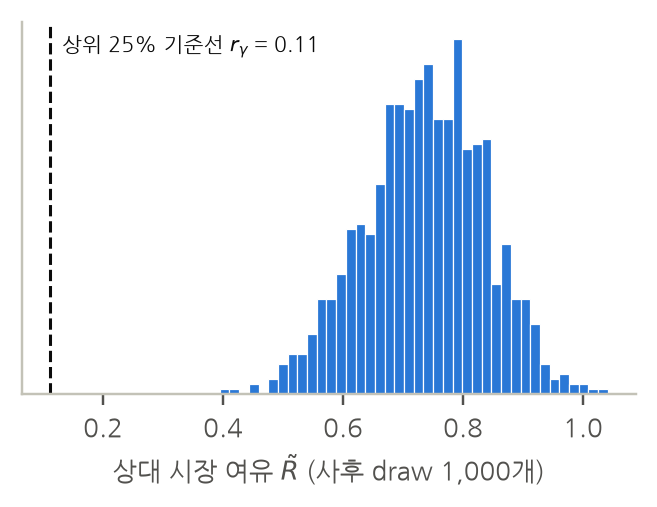
\includegraphics[width=0.92\linewidth]{figures/case_posterior.png}
\caption{경기도 과천시 중국음식의 상대 시장 여유 사후분포. 점선 오른쪽 면적이 확률 $v$다.}
\label{fig:case}
\end{figure}

\section{검증}
\subsection{수렴과 예측 보정}
4체인 $\times$ 4,000회 NUTS에서 최대 $\hat R$ 1.005, 최소 유효표본 bulk 592 / tail 993, 발산 0회로 수렴 기준($\hat R<1.01$, ESS $\ge400$, 발산 0)을 통과했다. 표~\ref{tab:cal}처럼 관측 셀이 사후예측 구간에 들어간 비율은 명목값과 거의 같다. 모형은 억제 셀 비율도 재현한다.

\begin{table}[t]
\centering
\caption{억제 재현과 사후예측 구간 포함률}
\label{tab:cal}
{\footnotesize\begin{tabular}{lrrrr}\toprule
업종 & 실제 억제 & 예측 억제 & 80\% 구간 & 90\% 구간 \\\midrule
한식 & 0.6\% & 1.2\% & 83\% & 90\% \\
중국음식 & 2.9\% & 1.8\% & 83\% & 91\% \\
일식회집 & 15.6\% & 13.6\% & 84\% & 91\% \\
서양음식 & 0.2\% & 0.1\% & 83\% & 91\% \\
스넥 & 2.2\% & 1.7\% & 84\% & 91\% \\
제과점 & 2.7\% & 2.7\% & 83\% & 91\% \\
편의점 & 0.0\% & 0.0\% & 83\% & 90\% \\
슈퍼마켓 & 1.2\% & 1.1\% & 83\% & 90\% \\
대형할인점 & 2.6\% & 2.4\% & 84\% & 91\% \\\bottomrule\end{tabular}}
\end{table}

\subsection{과거 점포 변화로 한 사후 점검}
판단표가 실제 점포 변화와 맞는지 과거 자료로 점검했다(그림~\ref{fig:retro}, 표~\ref{tab:retro}). 국세청 순증과의 상관은 대부분 평균회귀에서 나오므로 수요 정보가 없는 ``공급만'' 기준도 비슷한 값을 낸다. 어느 기간에서도 진입률을 예측하지 못했으므로 CREDO를 진입 예측기로 제시하지 않는다. 신규 점포 1년 생존으로 점검하면 수요 기간과 결과 기간의 시간 순서가 맞는다. 이 점검에서는 CREDO $\tilde R$만 구간이 0보다 크고(+0.075, 90\% 구간 +0.040--+0.115), 공급만 기준보다도 +0.043--+0.118 높다. 상관이 가장 강한 업종은 중국음식(+0.21)이다. 효과 크기가 작으므로 이를 ``생존 관점의 위험 선별''로 해석한다. 층 2 설계는 이 생존 점검 전에 확정했다.

\begin{figure*}[t]
\centering
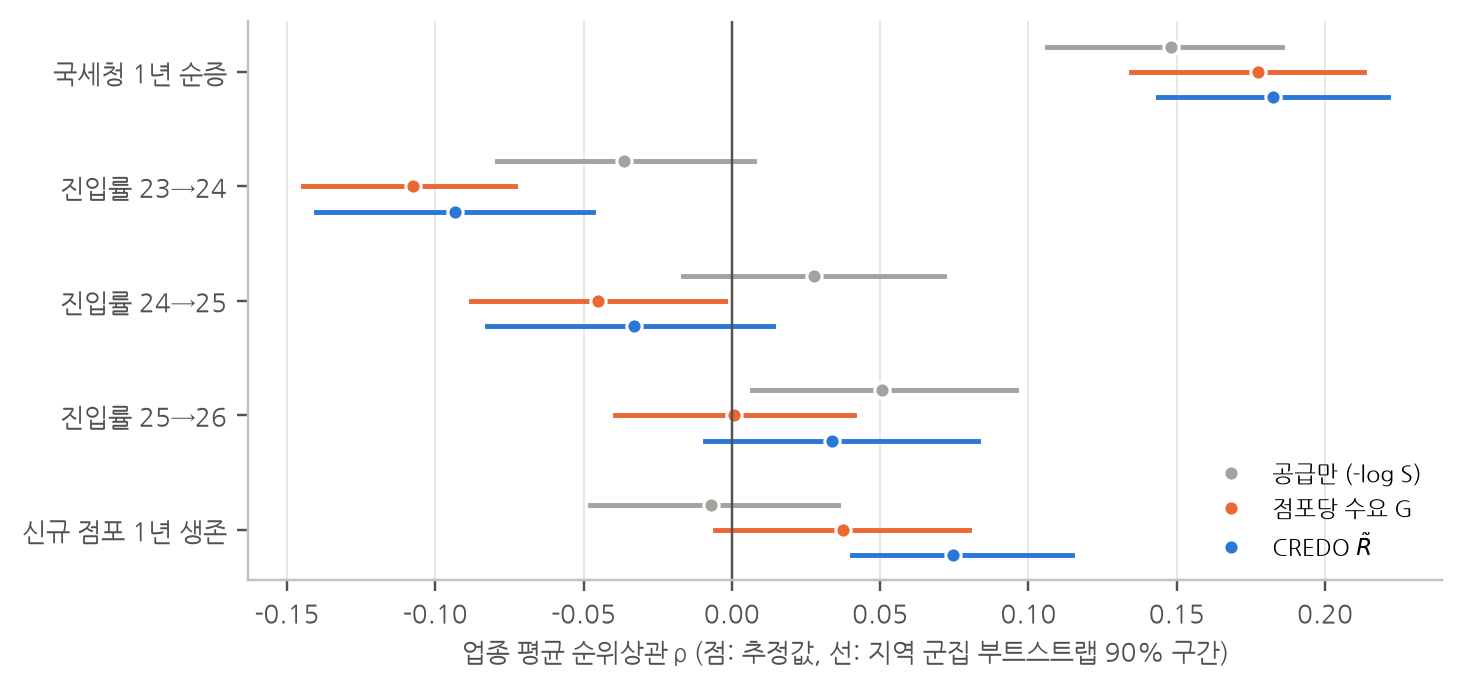
\includegraphics[width=0.82\textwidth]{figures/fig4_retro_validation.png}
\caption{과거 점포 변화와의 업종 평균 순위상관(점: 추정값, 선: 지역 군집 부트스트랩 90\% 구간).}
\label{fig:retro}
\end{figure*}

\begin{table}[t]
\centering
\caption{사후 점검 순위상관과 공급만 대비 차이(90\% 구간)}
\label{tab:retro}
{\setlength{\tabcolsep}{2pt}{\footnotesize\begin{tabular}{lrrrr}\toprule
결과변수 & 공급만 & 점포당 G & CREDO $\tilde R$ & $\tilde R$$-$공급만 \\\midrule
국세청 1년 순증 & +0.148 & +0.177 & +0.182 & [+0.004, +0.067] \\
상가정보 진입률 & +0.051 & +0.001 & +0.034 & [-0.049, +0.016] \\
신규 점포 1년 생존 & -0.007 & +0.037 & +0.075 & [+0.043, +0.118] \\\bottomrule\end{tabular}}}
\end{table}

\subsection{판단 규칙의 운영특성}
사후분포를 참값으로 두고 같은 목록 크기에서 규칙을 비교했다(표~\ref{tab:oc}). 점포당 수요 $G$로 만든 목록은 40\%--79\%가 어긋나지만 CREDO 목록의 오탐률은 9.5\%--9.9\%로 약속한 10\% 안에 있다. CREDO FDR 목록과 $\tilde R$ 사후평균 상위 $n$의 성능은 같다. 즉 성능 개선은 추정 대상 $\tilde R$에서 오고 FDR 규칙은 목록 길이를 정하고 오탐률 약속을 붙이는 역할을 한다. 이 비교는 표본 내 비교이므로 CREDO에 유리하다.

\begin{table}[t]
\centering
\caption{판단 규칙의 운영특성 (업종별 범위)}
\label{tab:oc}
{\footnotesize\begin{tabular}{lrr}\toprule
규칙 (같은 목록 크기) & 오탐률 & 적중률 \\\midrule
CREDO FDR 목록 & 9.5\%--9.9\% & 83.2\%--95.4\% \\
$\tilde R$ 사후평균 상위 $n$ & 9.6\%--9.9\% & 83.2\%--95.3\% \\
점포당 수요 G (지역 안) & 30.3\%--57.8\% & 42.0\%--66.8\% \\
점포당 수요 G & 39.9\%--79.5\% & 21.7\%--55.2\% \\\bottomrule\end{tabular}}
\end{table}

\subsection{강건성}
국세청 업종 대응을 넓혀도(한식에 기타음식점, 서양에 패스트푸드·커피 추가) 한식·스넥의 순위는 안정적이지만 서양음식·슈퍼마켓은 해석에 주의가 필요하다(표~\ref{tab:sens}). 4주 검증 후보는 팝업 관측오차를 1/4배--4배로 바꿔도 겹침이 0.82--1.00이다. 지역마다 BC카드 보유자의 연령 구성이 달라 생기는 편향을 점검하면 계수는 $\kappa=+2.57$(90\% 구간 +1.24--+3.91)로 가설 방향이지만 설명력이 1.6\%로 작다. 이 편향을 제거해도 상위 25\% 목록 겹침은 0.75--1.00이다. 상권수요 $\lambda$를 5·20km로 바꾸면 목적형 4업종의 순위상관은 0.95--0.99, 개설 목록 겹침은 0.82--0.93이다. 생존 순위상관도 +0.064($\lambda=5$), +0.076($\lambda=20$)로 주 분석과 비슷하다.

\begin{table}[t]
\centering
\caption{업종 대응표 확장 시 민감도}
\label{tab:sens}
{\footnotesize\begin{tabular}{lrrr}\toprule
업종 & 순위상관 & 상위 25\% 겹침 & 개설 목록 겹침 \\\midrule
한식 & 0.93 & 0.75 & 0.67 \\
서양음식 & 0.52 & 0.38 & 0.41 \\
스넥 & 0.78 & 0.56 & 0.58 \\
슈퍼마켓 & 0.70 & 0.43 & 0.42 \\\bottomrule\end{tabular}}
\end{table}

\section{서비스 설계}
판단표로 바로 구현할 수 있는 두 화면의 시안을 그림~\ref{fig:mock}에 담았다. 화면에 나온 지역, 수치, 선정 순서는 모두 실제 결과다.

\subsection{예비창업자 화면}
업종을 고르면 전국 지도에 개설 후보·4주 검증·보류가 표시된다. 지역을 누르면 판단 카드가 근거 문장, 확률, 순위 구간과 함께 나타난다. 서비스는 문장을 결과표에서 템플릿으로 생성하며 원자료를 외부 AI에 넣지 않는다. 검증 후보 지역에서는 팝업 매장·공유주방·단기 임대로 4주 매출을 확인한 뒤 결정하도록 안내한다. 검증 결과가 들어오면 같은 업종·인접 지역의 판단도 갱신한다.

\subsection{지원기관 화면}
예산으로 지원할 지역 수 $K$를 입력하면 대시보드가 식~\eqref{eq:cover}로 서로 겹치지 않는 $K$곳, 한 곳을 더할 때 늘어나는 커버 비율, 기대 커버 비율의 구간을 보여준다. 지원기관은 이를 창업 교육, 상권 컨설팅, 임차료 지원 대상 지역을 선정하는 데 쓸 수 있다.

\begin{figure*}[t]
\centering
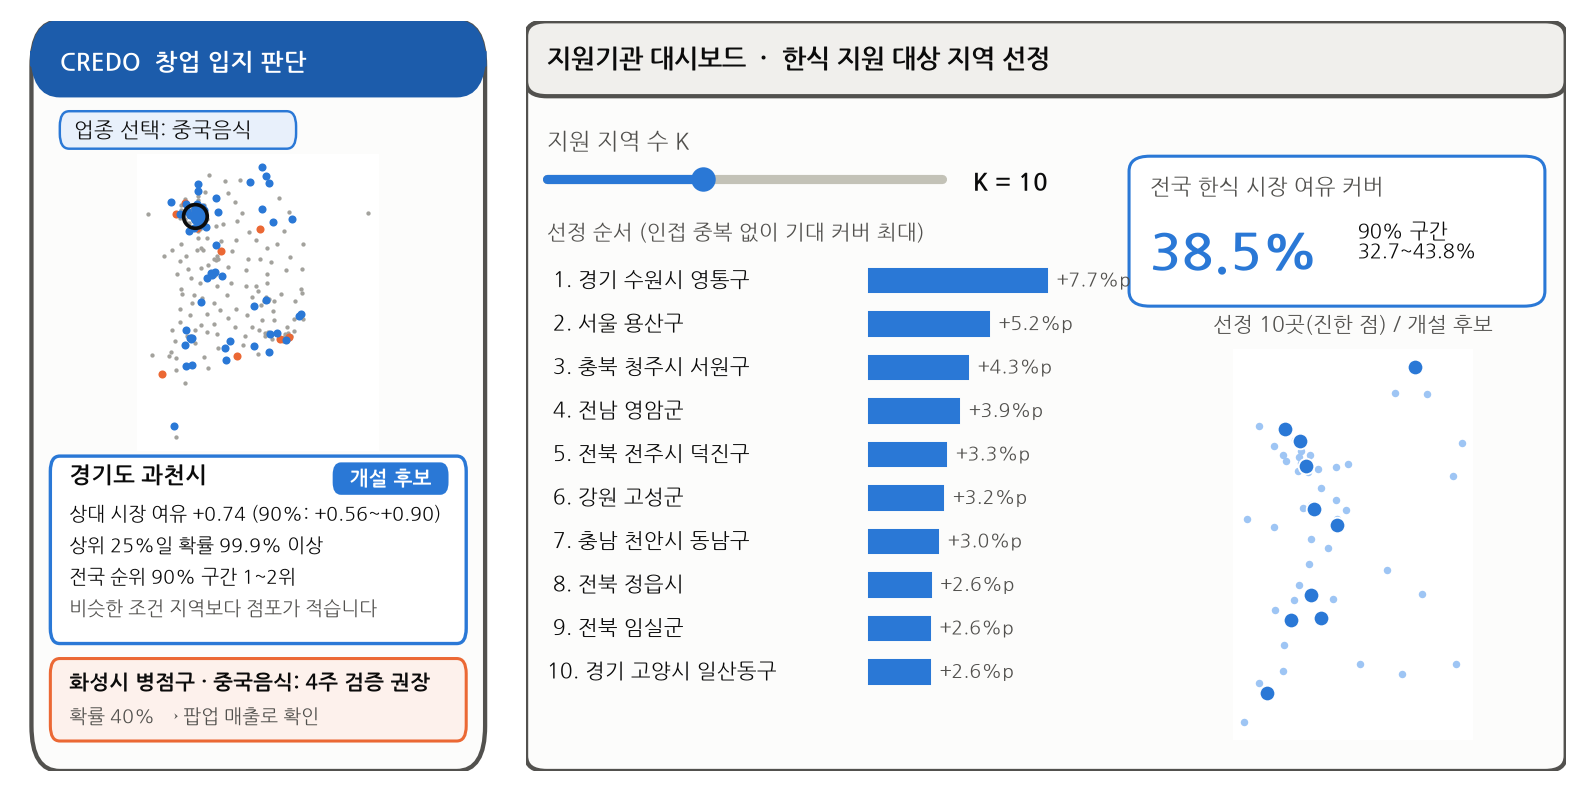
\includegraphics[width=\textwidth]{figures/mockup.png}
\caption{서비스 화면 시안. 왼쪽은 예비창업자 모바일 화면(판단 카드), 오른쪽은 지원기관 대시보드(한식 10곳 최적입지 선정).}
\label{fig:mock}
\end{figure*}

\subsection{활용 시나리오}
경기도에서 중국음식점을 준비하는 창업자를 예로 들면, 지도에서 경기도 과천시이 개설 후보로 표시된다. 판단 카드는 상위 25\%일 확률 99.9\% 이상와 전국 순위 구간 1--2위를 함께 보여주므로 창업자는 확신의 정도를 알고 임차 협상에 들어갈 수 있다. 같은 도의 경기도 화성시 병점구은 4주 검증 후보다. 서비스는 이곳에서 바로 계약하지 말고 공유주방이나 팝업으로 실제 매출을 먼저 확인하도록 권장한다. 확인한 매출은 인접 지역의 판단을 갱신하는 데 다시 쓰인다. 광역 지원기관은 대시보드에서 예산에 맞는 $K$를 정하면 서로 겹치지 않는 지원 대상 지역을 받는다. 이 선택이 덮는 시장 여유의 비율과 그 구간도 함께 나온다.

\subsection{운영}
BC카드 월별 집계와 국세청(월간)·상가정보(분기) 갱신에 맞춰 층 1--3을 다시 실행한다. 층 2·3은 수 분, 층 1은 GPU로 수 시간이 걸린다.

\section{기대효과와 사전 등록 검증}
비싼 임대료나 관광 유입 때문에 점포당 매출이 높아 보이는 곳이 있다. 임대료·유입을 통제하지 않은 점포당 수요로 입지를 고르면 이런 곳을 부족 지역으로 오인한다. CREDO는 그런 잘못된 진입 신호를 걸러내고 판단이 애매한 곳에서는 초기 자본을 투입하기 전에 4주 검증으로 정보를 얻게 한다. 판단표(decision\_table.csv, SHA-256 \texttt{d40fc74b4bd053d8}…)를 고정해 두고 국세청 2026-07·08 자료와 상가정보 2026-09 자료로 개설 후보 지역과 비후보 지역의 신규 점포 생존·진입을 비교할 예정이다\cite{Carree2007}.

\section{주요 설계 결정}
표~\ref{tab:decisions}에는 분석 중 내린 주요 결정과 그 근거를 정리했다. 결과를 본 뒤 유리한 설정을 고르지 않도록 층 2 모형은 신규 점포 생존 점검 전에 확정했다.

\begin{table}[t]
\centering
\caption{주요 설계 결정과 근거}
\label{tab:decisions}
{\footnotesize\setlength{\tabcolsep}{3pt}
\begin{tabular}{L{0.45\linewidth}L{0.47\linewidth}}
\toprule
결정 & 근거 \\\midrule
억제 기준을 데이터에서 유도하고 검사로 고정 & 업종·성별·월 최솟값이 모두 11 \\
한정식·갈비를 한식으로 합산 & 관측률 2.8\%·14.3\%, 국세청 한식음식점 범위와 일치 \\
대형할인점은 지원금 대조군으로만 사용 & 마트 없는 57개 군, 지원금 비적격 업종 \\
공급은 국세청 업종 이름 기준 1:1 대응 & 규모 통제 편상관 1위와 일치 \\
판단 지표는 지역 안 상대값 $\tilde R$ & $R$ 분산의 45\%가 지역 공통 성분 \\
시도 가구소득 제외 & 시군구 소비율 설명력 0.1--5.6\% \\
근로인구는 국민연금 가입자 & SGIS 사업체통계는 2019년까지 \\
합-0 centered 효과와 GPU NUTS & non-centered는 $\hat R$ 1.07로 실패 \\
지역 고정 공변량은 층 2로 & 층 1에서는 지역효과와 식별 불가 \\
근린형은 자기 지역, 목적형은 10km 감쇠 & 편의점 상권은 시군구보다 작음 \\
\bottomrule
\end{tabular}}
\end{table}

\section{한계}
분석 대상은 BC카드 관측 수요이며 전체 시장 매출이 아니다. 분석 기간 중 우리카드 독자망 전환으로 BC망 점유율이 하락했다. 지역별 점유율 차이는 $\tilde R$로 상쇄하지만 업종별 점유율 차이는 남는다. 지역 기준과 억제 기준은 공식 코드북이 아닌 데이터로 추정했다. 사후 점검에는 과거 1년 자료를 썼다. 생존 연관의 효과 크기는 작고 진입은 예측하지 못했다. 층 2는 6개월 횡단면으로 2단계 추정을 하므로 점포 수의 내생성이 남는다. 서양음식·슈퍼마켓은 업종 대응에 따라 순위가 흔들린다.

\section{결론}
CREDO는 BC카드 결제 데이터의 억제, 균형 착시, 불확실성 문제를 세 층으로 나눠 다루고 결과를 전국 255개 시군구 $\times$ 8개 업종의 개설·검증·보류 판단과 공간 최적입지 선정으로 제시한다. 추천 목록에는 기대 오탐률 10\% 이하라는 약속이 붙는다. 판단이 애매한 곳은 비용이 큰 결정 전에 검증을 거친다. 사전 등록한 판단표는 공개 예정인 국세청·상가정보 자료로 다시 검증한다.

\begin{thebibliography}{10}
\bibitem{Bresnahan1991}
T.~F. Bresnahan and P.~C. Reiss, ``Entry and competition in concentrated markets,'' \emph{J. Polit. Econ.}, vol.~99, no.~5, pp.~977--1009, 1991.
\bibitem{Nemhauser1978}
G.~L. Nemhauser, L.~A. Wolsey, and M.~L. Fisher, ``An analysis of approximations for maximizing submodular set functions---I,'' \emph{Math. Program.}, vol.~14, pp.~265--294, 1978.
\bibitem{BerryWaldfogel1999}
S. Berry and J. Waldfogel, ``Free entry and social inefficiency in radio broadcasting,'' \emph{RAND J. Econ.}, vol.~30, no.~3, pp.~397--420, 1999.
\bibitem{Muller2004}
P. M\"uller, G. Parmigiani, C. Robert, and J. Rousseau, ``Optimal sample size for multiple testing: The case of gene expression microarrays,'' \emph{J. Amer. Statist. Assoc.}, vol.~99, pp.~990--1001, 2004.
\bibitem{ShenLouis1998}
W. Shen and T.~A. Louis, ``Triple-goal estimates in two-stage hierarchical models,'' \emph{J. Roy. Statist. Soc. B}, vol.~60, pp.~455--471, 1998.
\bibitem{Lin2006}
R. Lin, T.~A. Louis, S.~M. Paddock, and G. Ridgeway, ``Loss function based ranking in two-stage hierarchical models,'' \emph{Bayesian Anal.}, vol.~1, no.~4, pp.~915--946, 2006.
\bibitem{Frazier2008}
P.~I. Frazier, W.~B. Powell, and S. Dayanik, ``A knowledge-gradient policy for sequential information collection,'' \emph{SIAM J. Control Optim.}, vol.~47, no.~5, pp.~2410--2439, 2008.
\bibitem{Hoffman2014}
M.~D. Hoffman and A. Gelman, ``The No-U-Turn sampler,'' \emph{J. Mach. Learn. Res.}, vol.~15, pp.~1593--1623, 2014.
\bibitem{Schaumans2015}
C. Schaumans and F. Verboven, ``Entry and competition in differentiated products markets,'' \emph{Rev. Econ. Stat.}, vol.~97, no.~1, pp.~195--209, 2015.
\bibitem{Carree2007}
M. Carree and M. Dejardin, ``Entry thresholds and actual entry and exit in local markets,'' \emph{Small Bus. Econ.}, vol.~29, pp.~203--212, 2007.
\end{thebibliography}

\end{document}
